% Created 2017-04-12 Wed 19:01
% Intended LaTeX compiler: pdflatex
\documentclass[12pt]{article}
\usepackage[utf8]{inputenc}
\usepackage[T1]{fontenc}
\usepackage{graphicx}
\usepackage{grffile}
\usepackage{longtable}
\usepackage{wrapfig}
\usepackage{rotating}
\usepackage[normalem]{ulem}
\usepackage{amsmath}
\usepackage{textcomp}
\usepackage{amssymb}
\usepackage{capt-of}
\usepackage{hyperref}
\usepackage[margin=1.0in]{geometry}
\documentclass{article}
\usepackage{setspace,mathrsfs,amsmath,amsthm,amssymb,graphicx,cancel,lmodern,mathtools}
\author{Justen Rickert}
\date{\today}
\title{Math3283W study guiding}
\hypersetup{
 pdfauthor={Justen Rickert},
 pdftitle={Math3283W study guiding},
 pdfkeywords={},
 pdfsubject={},
 pdfcreator={Emacs 26.0.50.1 (Org mode 9.0.5)}, 
 pdflang={English}}
\begin{document}

\maketitle
\tableofcontents

\newcommand\bd[1]{\text{bd }#1}
\newcommand\cl[1]{\text{cl }#1}
\newcommand\int[1]{\text{int }#1}
\newcommand\lim[1]{\text{lim }#1}
\newcommand{\def}[1]{\textit{\textbf{#1}}}
\newcommand\abs[1]{\left|#1\right|}
\newcommand\deg{\textdegree}
\newcommand\Real{\mathbb{R}}
\newcommand\Natural{\mathbb{N}}
\newcommand\Rational{\mathbb{Q}}
\newcommand\sube{\subseteq}
\newcommand\supe{\supseteq}
\newcommand\sub{\subset}
\newcommand\sup{\supset}
\newcommand\setm{\setminus}
\newcommand\pr{\ensuremath{'}}
\newcommand\R{\mathcal{R}}
\newcommand\calR{\mathcal{R}}
\newcommand\calP{\mathcal{P}}
\newcommand\pow{\mathscr{P}}
\newcommand\indX{\mathscr{X}}
\newcommand\F{\mathscr{F}}
\newcommand\G{\mathscr{G}}
\newcommand\nil{\varnothing}

\theoremstyle{definition}
\newtheorem{definition}{Definition}
\renewcommand\qedsymbol{$\blacksquare$}

\newtheorem{lemma}[Theorem]{lemma}
\theoremstyle{definition}
\newtheorem{definition}{Def}[section]
\newtheorem*{remark}{Remark}
\newtheorem*{corollary}{Corollary}

\section{Midterm one}
\label{sec:org96a272d}
\subsection{Vocabulary}
\label{sec:org687136d}
\subsubsection{Section 1.1}
\label{sec:org98d475a}
\begin{description}
\item[{statement}] A sentence classified as something either true or false is a
\emph{statement}.
\item[{sentential connectives}] \emph{not}, \emph{and}, \emph{or}, \emph{if\dots{} then}, \emph{if and only if}.
\begin{description}
\item[{conjunction}] \(p\land{}q\)
\item[{disjunction}] \(p\lor{}q\)
\item[{implication/conditional}] \(p\Rightarrow{}q\)
\begin{description}
\item[{antecedant}] \(p\) statement
\item[{consequent}] \(q\) statement
\end{description}
\item[{biconditional}] \(p\Leftrightarrow{}q\)
\item[{negation}] \(\neg{}p\) represents the logical opposite of \(p\).
\end{description}
\item[{tautology}] A statement which is true in all cases.
\begin{itemize}
\item examples:
\end{itemize}
\end{description}
\begin{center}
\(\neg(p\land{}q)\Leftrightarrow[(\neg{}p)\lor(\neg{}q))]\) \\
\(\neg(p\lor{}q)\Leftrightarrow[(\neg{}p)\land(\neg{}q))]\) \\
\(\neg(p\Rightarrow{}q)\Leftrightarrow[p\lor(\neg{}q)]\) \\
\end{center}

\subsubsection{Section 1.2}
\label{sec:orge97f605}
\begin{description}
\item[{universal quantifier}] \(\forall{}x,p(x)\)
\item[{existential quantifier}] \(\exists{}x\ni{}p(x)\)
\end{description}

\subsubsection{Section 1.3}
\label{sec:orgb71e36c}
\begin{description}
\item[{deductive reasoning}] Applying a general principle to a particular case.
\item[{\(p\Rightarrow{}q\) as a theorem}] When an implication is identified as a theorem, it is
customary to refer to \(p\) as the \textbf{hypothesis} and \(q\) as the \textbf{conclusion}.
\item[{converse}] \(p\Rightarrow{}q\) has the converse \(q\Rightarrow{}p\). Not tautologically equivalent to
implication.
\item[{inverse}] \(p\Rightarrow{}q\) has the inverse \((\neg{}p)\Rightarrow{}(\neg{}q)\). Not tautologically
equivalent to implication.
\item[{contrapositive}] Tautologically equivalent to the implication.
\end{description}
\begin{center}
\((p\Rightarrow{}q)\Leftrightarrow(\neg{}q\Rightarrow{}\neg{}p)\)
\end{center}

\subsubsection{Section 2.1}
\label{sec:org3fc2d2a}
\begin{description}
\item[{subset}] \(A\sube{}B\). \(A\) is a \textbf{subset} of \(B\) (or \(A\) is \textbf{contained} in \(B\)). If we
want to prove \(A\sube{}B\), then we must prove "if \(x\in{}A\), then \(x\in{}B\)".
\begin{description}
\item[{proper subset}] \(A\sub{}B\). \(\forall{}a\in{}A, a\in{}B\), but \(\exists{}b\in{}B\ni{}b\notin{}A\). That is, all elements
of \(A\) are in \(B\), but some elements of \(B\) are not in \(A\).
\item[{equal}] A set \(A\) is equal to a set \(B\) provided that \(A\sube{}B\) and \(A\supe{}B\) (or
\(A\sube{}B\) and \(B\sube{}A\)).
\end{description}
\item[{closed interval}] \([a,b]\)
\item[{open interval}] \((a,b)\)
\item[{half--open (half--closed) interval}] \([a,b)\), or \((a,b]\).
\item[{union}] \(A\cup{}B=\{x\mid{}x\in{}A\) or \(x\in{}B\}\)
\item[{intersection}] \(A\cap{}B=\{x\mid{}x\in{}A\) and \(x\in{}B\}\)
\begin{itemize}
\item If \(A\cap{}B=\varnothing\), then \(A\) and \(B\) are said to be \textbf{disjoint}
\end{itemize}
\item[{complement}] \(A\setminus{}B=\{x\mid{}x\in{}A\) and \(x\notin{}B\}\)
\end{description}

\subsubsection{Section 2.2}
\label{sec:org0a52a8c}
\begin{description}
\item[{ordered pairs}] \((a,b)=\{\{a\},\{a,b\}\}\)
\item[{Cartesian product (cross product)}] \(A\times{}B=\{(a,b)\mid{}a\in{}A\) and \(b\in{}B\}\)
\item[{relation}] A \textbf{relation} between \(A\) and \(B\) is any subset \(\R\) of \(A\times{}B\). We say
that an element a in \(A\) is related by \(\R\) to an element in \(b\) in
\(B\) if \((a,b)\in{}\R\). The first set \(A\) is referred to as the \textbf{domain},
of the relation and denoted dom \(\R\). If \(B=A\), then we speak of a
relation \(\R\sube{}A\times{}A\) being a \textbf{relation on} \(A\).
\begin{description}
\item[{equivalence relation}] A relation \(\R\) is an \textbf{equivalence relation} if:
\begin{enumerate}
\item \(x\R{}x\) \hfill (reflexive property)
\item If \(x\R{}y\), then \(y\R{}x\) \hfill (symmetric property)
\item If \(x\R{}y\) and \(y\R{}z\), then \(x\R{}z\) \hfill (transitive property)
\end{enumerate}
\item[{equivalence class}] An equivalence class (with respect to \(\R\)) of \(x\in{}S\) is
defined to be the set
\begin{center}
\(E_{x}=\{y\in{}S\mid{}y\R{}x\}\)
\end{center}
\begin{description}
\item[{partition}] Also, we see that an equivalence relation \(\R\) on a set \(S\)
breaks \(S\) into \textbf{disjoint} pieces in a natural way. A partition
of a set \(S\) is a collection \(\pow\) of nonempty subsets of
\(S\) such that
\begin{enumerate}
\item Each \(x\in{}S\) belongs to some subset \(A\in\pow\).
\item For all \(A,B\in\pow\), if \(A\ne{}B\), then \(A\cap{}B=\nil\).
\end{enumerate}
\end{description}
A member of \(\pow\) is called a \textbf{piece} of the partition.
\end{description}
\end{description}

\subsubsection{Section 2.3}
\label{sec:org45d01fa}
\begin{description}
\item[{function}] Let \(A\) and \(B\) be sets. Then, a \textbf{function} from \(A\) to \(B\) is a
nonempty relation \(f\sube{}A\times{}B\) that satisfies the following two
conditions.
\begin{enumerate}
\item \emph{Existence}: For all \(a\) in \(A\), there exists a \(b\) in \(B\) such that
\((a,b)\in{}f\).
\item Uniqueness: If \((a,b)\in{}f\) and \((a,c)\in{}f\), then \(b=c\).
\end{enumerate}
Set A is called the \textbf{domain} of \(f\) and is denoted by dom \(f\). Set \(B\) is
            referred to as the \textbf{codomain} of \(f\). We may write
            \(f:A\longrightarrow{}B\) to indicate that \(f\) has domain A and
            codomain \(B\).
\item[{range}] The set of all second elements of members of \(f\). That is:
\begin{center}
rng \(f = \{b\in{}B\mid{}\exists{}a\in{}A\ni(a,b)\in{}f\}\)
\end{center}
\item[{surjective (A onto B)}] A function \(f:A\longrightarrow{}B\) is \textbf{surjective} if
\(B=\) rng \(f\). \(f\) is referred to as a \textbf{surjection}.
\item[{injective (one-to-one)}] A function \(f:A\longrightarrow{}B\) is \textbf{injective} if,
for all \(a\) and \(a\pr\) in \(A\), \(f(a)=f(a\pr)\). \(f\) is referred to as an
\textbf{injection}.
\item[{bijective}] A function \(f:A\longrightarrow{}B\) is bjective or a bijection if
it is both surjective and injective.
\item[{characteristic function (indicator function)}] Let \(A\) be a nonempty set and
let \(S\) be a subset of \(A\). We may define a function
\(\indX_S:A\longrightarrow{}\{0,1\}\) by
\[\indX_S(a)= 
  \begin{cases} 
    1 & $if $x\in{}S,  \\
    0, & $if $x\notin{}S.
  \end{cases} \]
If \(S\) is a nonempty proper subset of \(A\), then \(\indX_S\) is surjective. If
   \(S=\nil\) or \(S=A\), then \(\indX_S\) is not surjective.
\item[{vertical line test}] 

\item[{inverse}] Let \(f:A\longrightarrow{}B\) be bijective. The \textbf{inverse function} of
\(f\) is the function \(f^{-1}\) given by
\begin{center}
\(f^{-1}=\{(y,x)\in{}B\times{}A\mid(x,y)\in{}f\}\).
\end{center}
\item[{identity function}] A function defined on a set A that maps each element in A
onto itself is called the \textbf{identity function} on \(A\), and is denoted
\(f^{-1}\circ{}f=i_{A}\). Furthermore, if \(f(x)=y\), then \(x=f^{-1}(y)\), so that
\begin{center}
\(f\circ{}f^{-1}(y)=f(f^{-1}(y))=f(x)=y\).
\end{center}
Thus, \(f\circ{}f^{-1}=i_{B}\).
\end{description}
\subsection{Theorem}
\label{sec:org289bae6}
\subsubsection{Section 1.4}
\label{sec:org89beb80}
\begin{itemize}
\item This example shows a \emph{direct proof}.
\begin{itemize}
\item For every \(\epsilon>0\) there exists a \(\delta>0\) such that
\end{itemize}
\begin{center}
\(1-\delta<x<1+\delta\) implies that \(5-\epsilon<2x+3<5+\epsilon\).
\end{center}

\begin{enumerate}
\item Begin by letting \(\epsilon\) be an arbitrary positive number, i.e. \(\epsilon>0\). We need to
use this \(\epsilon\) to find a positive \(\delta\) with the property that
\begin{center}
\(1-\delta<x<1+\delta\) implies that \(5-\epsilon<2x+3<5+\epsilon\).
\end{center}
\item Given any \(\epsilon>0\), let \(\delta=\epsilon/2\). \(\delta>0\), and whenever
$$1-\delta<x<1+\delta$$
we have $$1-\frac{\epsilon}{2}<x<1+\frac{\epsilon}{2}$$
so that $$2-\epsilon<2x<2+\epsilon$$
and $$5-\epsilon<2x+3<5+\epsilon$$
thus \\ 
\center $1-\delta<x<1+\delta$ implies that $5-\epsilon<2x+3<5+\epsilon$.
\end{enumerate}
\item This example shows a \emph{indirect proof}.
\begin{itemize}
\item Let \(f\) be an integrable function, so that
\end{itemize}
\begin{center}
If \(\int_{0}^{1}f(x)dx\neq0\), then there exists a point \(x\) in the interval \([0,1]\) such
that \(f(x)\neq0\).
\end{center}

\begin{enumerate}
\item Symbolically, we have \(p\Rightarrow{}q\), where
\begin{center}
$$p: \int_{0}^{1}f(x)dx\neq0,$$ \\
\(q: \exists{}x\) in \([0,1]\ni{}f(x)\neq0\).
\end{center}

The contrapositive implication, \(\neg{}q\Rightarrow{}\neg{}p\), can be written
\begin{center}
If for every \(x\) in \([0,1]\), \(f(x)=0\), then \(\int_{0}^{1}f(x)dx=0\).
\end{center}
\item This is obviously true. The integral of all 0 integrands is obviously 0.
\end{enumerate}
\item This example shows a \emph{proof by contradiction}.
\begin{itemize}
\item Let \(x\) be a real number.
\end{itemize}
\begin{center}
If \(x>0\), then \(1/x>0\).
\end{center}

\begin{enumerate}
\item Symbolically, we have \(p\Rightarrow{}q\), where
\begin{center}
\(p: x>0\) \\
\(q: 1/x>0\) \\
\end{center}

so that, \((p\Rightarrow{}q)\Leftrightarrow{}((p\land{}\neg{}q)\Rightarrow{}c)\), where \(c\) represents a contradiction.
\item Begin by supposing \(x>0\) and \(1/x\le0\). Since \(x>0\), we can multiply both
sides of the inequality \(1/x\le{}0\) by \(x\) to obtain
\begin{center}
$$(x)\left(\frac{1}{x}\right)\le(x)(0)$$
\end{center}

But \((x)(1/x)=1\) and \((x)(0)=0\), so we have \(1\le0\), a contradiction to the
(presumably known) fact that \(1>0\). Having show that \(p\land{}\neg{}q\) leads to a
contradiction, we conclude that \(p\Rightarrow{}q\).
\end{enumerate}
\item This example shows a \emph{proof with absolute value}.
\begin{itemize}
\item If \(x\) is a real number, then \(x\le\abs{x}\)
\end{itemize}
\begin{center}
\(s: x\) is a real number \\
\(r: x\le\abs{x}\) \\
\end{center}

The definition of statement \(r\) can be rewritten as:
\[\lvert{}x\rvert{}= 
  \begin{cases} 
    x & $if $x\ge{}0,  \\
    -x, & $if $x<0.
  \end{cases} \]

\begin{enumerate}
\item Since the definition is divided into two parts, it is natural to divide our
proof into two cases. Thus statement \(s\) is replaced by the equivalent
disjunction \(p\lor{}q\), where
\begin{center}
\(p: x\ge0\) and \(q: x<0\).
\end{center}

\item The case to prove now is \((p\lor{}q)\Rightarrow{}r\), which is the same as \((p\Rightarrow{}r)\land(q\Rightarrow{}r)\).

\item If \(x\ge0\), then \(x=\lvert{}x\rvert{}\). If \(x<0\), then \(-x>0\), so that
\(x<0<-x=\lvert{}x\rvert{}\). Or, \(x\le\abs{x}\). Thus, \((p\Rightarrow{}r)\land(q\Rightarrow{}r)\). Hence, if
\(x\) is a real number, then \(x\le\abs{x}\)
\end{enumerate}
\end{itemize}
\subsubsection{Section 2.3}
\label{sec:orgc030704}
\begin{itemize}
\item Let \(f:A\longrightarrow{}B\). Then
\begin{enumerate}
\item \(f^{-1}:B\longrightarrow{}A\) is bijective.
\item \(f^{-1}\circ{}f=i_{A}\) and \(f\circ{}f^{-1}=i_{B}\).
\end{enumerate}
\end{itemize}
\subsection{Practice test}
\label{sec:orgbf97938}
\begin{itemize}
\item question (1, d)
\begin{itemize}
\item Define \(A_{n}=(3,4+\frac{1}{n})\), an open interval in \(\Real\), for each natural
number \(n\). Without writing a proof, determine $$\bigcap\limits_{n=1}^{\infty}A_{n}$$.
\end{itemize}
\end{itemize}
\textbf{answer}: When \(n=1\), \(A_{1}=(3,4+1)=(3,5)\). When \(n=2\), the
\(A_{1}=(3,4+\frac{1}{2})=(3,4.5)\). Here, consider \(f(n)=4+\frac{2}{n}\), the
function for the upper bound of \(A_{n}\) for each \(n\). Here, the forward difference
quotient \(\Delta{}f(1)=f(2)-f(1)=4.5-5<0\). Considering the function \(f(n)\), this
difference quotient will always be negative. Therefore, the highest upper bound
over all the parts of the union will be \(f(1)=5\). Since the lower bound function
is constant, the lowest lower bound over all the parts of the union will be 3.
Therefore, \(A_{n}\sube{}(3,5)\), and \(A_{n}=\{(3,4+\frac{1}{n})\mid{}n\in{}\Natural\}\).

\begin{itemize}
\item question (2, a) For all \(x\), there exists \(y\) such that for all \(z\), if \(y<x\)
then \(z<y\).
\begin{enumerate}
\item write the negation:
\item Determine whether the original statement is true or false. Write "true" or
"false", and then justify your answer by proving the original statment or
the negation that you wrote in (a):
\end{enumerate}
\end{itemize}
\textbf{answer 1}: There exists \(x\) such that for all \(y\), there exists \(z\) such that
\(y<x\) and \(z\ge{}y\). \\
\textbf{answer 2}: Let \(x\) be some constant \(x_{0}\), such that \(y<x_{0}\) for all y. Since this
\(y\) can be any of all the numbers in \(\Real\), say \(y\ge{}x_{0}\), the statement \(y<x_{0}\)
is not true. Given a conjunction of a false statement and any other statement,
the conjunction is false. Since this statement is the negation of the original
statement and false, the original statement must be true. \\

\begin{itemize}
\item question (3,a)
\begin{enumerate}
\item Suppose that \(A=\{1,2,3\}\), \(B=\{4,5\}\), and \(C=\{6,7,8\}\). Let \(R\) be the
relation on \(A\times{}C\) given by \(\{(1,7),(3,6),(3,7)\}\) and \(S\) by the relation
on \(B\times{}C\) given by \(\{(4,7),(4,8),(5,6)\}\). Find \(S^{-1}\circ{}R\).
\item Given \(R\) a relation on \(A\times{}B\) and \(S\) a relation on \(B\times{}C\), prove that
\((S\circ{}R)^{-1}=R^{-1}\circ{}S^{-1}\).
\item Suppose that A and B are non-empty sets. Prove that \(A\times{}B=B\times{}A\) if and only
if \(A=B\).
\end{enumerate}
\end{itemize}
\textbf{answer 1}: Since \(S\) is defined, and \(S^{-1}=\{(c,b)\in{}C\times{}B\mid{}(b,c)\in{}S\}\),
\(S^{-1}=\{(7,4),(8,4),(6,5)\}\). Then,
\(S^{-1}\circ{}R=\{(7,4),(8,4),(6,5)\}\circ\{(1,7),(3,6),(3,7)\}\). This can be
simplified to \(S^{-1}\circ{}R=\{(1,4),(3,5),(3,4)\}\). \\
\textbf{answer 2}: Consider \(a\in{}A\), \(b\in{}B\), and \(c\in{}C\). \(S\circ{}R\) is a relation such that
\((a,c)\in{}S\circ{}R\sube{}A\times{}C\). Thus, \((S\circ{}R)^{-1}=\{(c,a)\in{}C\times{}A\mid{}(a,c)\in{}S\circ{}R\}\).

Given \((a,b)\in{}R\), by definition of Inverse \(R^{-1}=\{(b,a)\in{}B\times{}A\mid{}(a,b)\in{}R\}\).
Given \((b,c)\in{}S\), by definition of Inverse \(S^{-1}=\{(c,b)\in{}C\times{}B\mid{}(b,c)\in{}S\}\).
Then,
\(R^{-1}\circ{}S^{-1}=\{(c,a)\in{}C\times{}A\mid{}\exists{}b\in{}B\ni{}(a,b)\in{}R\land{}(b,c)\in{}S\}\).
However, this is the same as
\(R^{-1}\circ{}S^{-1}=\{(c,a)\in{}C\times{}A\mid{}(a,c)\in{}S\circ{}R\}\), by the
definition of Cartesian Product.

Thus, since \((S\circ{}R)^{-1}\) and \(R^{-1}\circ{}S^{-1}\) have the same definitions, it must be
that \((S\circ{}R)^{-1}=R^{-1}\circ{}S^{-1}\).

\textbf{answer 3}: (\(\Leftarrow\)) Let \(A=B\). It must be that \(A\times{}B=B\times{}A\), as having both leads to
\(B\times{}B=B\times{}B\) or \(A\times{}A=A\times{}A\) which are true. \\
(\(\Rightarrow\)) Let \(A\times{}B=B\times{}A\), and remember \(A\) and \(B\) are non-empty sets. By definition,
\(A\times{}B=\{(a,b)\mid{}a\in{}A\land{}b\in{}B\}\). Just as well, by definition,
\(B\times{}A=\{(b,a)\mid{}a\in{}A\land{}b\in{}B\}\). Having this implies that for every \((a,b)\in{}A\times{}B\) and
the corresponding \((b,a)\in{}B\times{}A\), \((a,b)=(b,a)\). Thus, \(A=B\). \\
In sum, this means \(A\times{}B=B\times{}A\) if and only if \(A=B\).

\begin{itemize}
\item question (4, a) Prove which one is true and which one is false.
\begin{itemize}
\item For all subsets \(S\) and \(T\) of a universal set \(U\), we have \(U\setminus(S\setminus{}T)\sube(U\setminus{}S)\cup{}T\).
\item For all subsets \(S\) and \(T\) of a universal set \(U\), we have \(U\setminus(S\setminus{}T)\sube(U\setminus{}S)\cap{}T\).
\end{itemize}
\end{itemize}
\textbf{answer}: The first statement to consider, \(U\setminus{}S\), has definition
\(U\setminus{}S=\{u\in{}U\mid{}u\notin{}S\}\). Then \((U\setminus{}S)\cup{}T=\{u\in{}U\mid{}u\notin{}S\}\cup\{u\in{}T\}\). Which is to say
that \(u\in{}U\), \(u\notin{}S\), and \(u\in{}T\), so that \((U\setminus{}S)\cup{}T=\{u\mid{}u\in{}U\land{}u\notin{}S\land{}u\in{}T\}\). \\
Consider the next statement \(A\), in particular \(U\setminus(S\setminus{}T)\). By definition
\(S\setminus{}T=\{u\in{}S\mid{}u\notin{}T\}\). By definition, again, \(U\setminus{}(S\setminus{}T)=\{u\in{}U\mid{}u\notin{}(S\setminus{}T)\}\),
that is \(U\setminus{}(S\setminus{}T)=\{u\in{}U\mid{}u\notin{}S\land{}u\in{}T)\}\). Which is to say that \(u\in{}U\), \(u\notin{}S\), and
\(u\in{}T\), so that \(U\setminus{}(S\setminus{}T)=\{u\mid{}u\in{}U\land{}u\notin{}S\land{}u\in{}T\}\). \\
Thus, statement A, \(U\setminus(S\setminus{}T)\sube(U\setminus{}S)\cup{}T\), is the true statement.
\begin{itemize}
\item question (4, b) Give a counterexample to the false statement, where \(U=\Real\),
and \(S\) and \(T\) are open interval in \(\Real\).
\end{itemize}
\textbf{answer}: Let subset \(S=\{x\in\Real\mid{}x>1\}\), and \(T=\{x\in\Real\mid{}x<1\}\). \(S\)
and \(T\) are disjoint, meaning \(U\setminus{}(S\setminus{}T)=U\setminus{}S\). So, we have \(U\setminus{}S\sube{}(U\setminus{}S)\cap{}T\). By
definition of set intersection, \((U\setminus{}S)\cap{}T=\{x\in\Real\mid{}x\in{}(U\setminus{}S)\land{}x\in{}T\}\), where
\(U\setminus{}S=\{x\in\Real\mid{}x\in{}U\land{}x\notin{}S\}\). Here, we have \(U\setminus{}S=\{x\in\Real\mid{}x\le{}1\}\), and
\((U\setminus{}S)\cap{}T=\{x\in\Real\mid{}x\le1\land{}x<1\}\) which is \((U\setminus{}S)\cap{}T=\{x\in\Real\mid{}x<1\}\). Just
as well, it can be seen that \(U\setminus(S\setminus{}T)\supe(U\setminus{}S)\cap{}T\), which is sort of the opposite of
the statement B.
\begin{itemize}
\item question (5) Prove that, for all integers \(p\) and \(q\), if \(pq\) is an even
integer, then \(p\) is an even integer or \(q\) is an even integer.
\end{itemize}
\textbf{answer}: Consider the contrapositive of the predicate in the statement: For all
integers \(p\) and \(q\), if \(p\) is an odd integer and \(q\) is an odd integer, then
\(pq\) is an odd integer. Let \(p=2k-1\) and \(q=2k-1\), for integers \(k\). Then, it is
straightforward that \(pq=(2k-1)(2k-1)=4k^{2}-4k+1=2(2k^{2}-2k)+1=2j+1\) for some
integer \(j=2k^{2}-2k\) and is therefore odd. Thus, "for all integers \(p\) and \(q\), if
\(p\) and \(q\) are odd integers, then \(pq\) is an odd integer" being true means that
its contrapositive is true, i.e. "for all integers \(p\) and \(q\), if \(pq\) is an
even integer, then \(p\) is an even integer or \(q\) is an even integer" is true.
\section{Midterm two}
\label{sec:orgef53c91}
\subsection{The Real Numbers}
\label{sec:org92372f3}
\begin{definition}{Well-ordering property of $\Natural$}
  If $S$ is a nonempty subset of $\Natural$, then there exists an element $m \in
  S$ such that $m \le k$ for all $k \in S$.
\end{definition}

\begin{definition}{Mathematical Induction}
  A technique of mathematical proof.
  \begin{enumerate}
  \item $P(1)$ is true
  \item Whenever $P(k)$ is true, for some number $k$, then $P(k+1)$ is true.
  \item Proof by contradiction :: Given statements $P(n)$, $n\in\Natural$. Show
    if we have properties 1) and 2), then $P(n)$ holds for all $n$. Suppose
    $P(n)$ false for some $n$. Let $F=\{n\in\Natural : P(n) \text{ false}\}$.
    $F$ is non-empty by assumption, so by well-ordering principle it has a least
    element, say $n_{0}\ne{}1$. Consider $n_{0}-1$, a natural number, so that
    $P(n_{0}-1)$ is true, since otherwise $n_{0}$ wasn't the smallest element of
    $F$.
  \end{enumerate}
  \textit{Slight Generalization}: --- want to prove $p(n)$ for all $n\ge n_0$,
  then prove:
  \begin{enumerate}
     \item $p(n_0$) is true.
     \item if $p(k)$ is true for $k$, then $p(k+1)$ is true with $k\ge n_0$
  \end{enumerate}
\end{definition}

\subsubsection{Examples}
\label{sec:org231ec8f}
\begin{itemize}
\item \uline{Example}: For which \(n\) is \(n!>n^{n}\)?

Expect \(n!>2^n\) if \(n\ge{}4\). (i.e. for all \(n\ge{}4\)).

Base case: True if \(n_{0}=4\) since \(24>16\). Suppose \(k!>2^{k}\). 

Inductive step: Show: \((k+1)!>2^{k+1}\). \uline{Easy}: $$k!>2^{k} \Rightarrow
      (k+1)!>2^{k}(k+1)>2^{k+1}$$ since \(k+1>2\) if \(k\ge{}4\).

\item \uline{Example}: For \(n\ge3\), if we connect \(n\) points on circle \(w\) with straight
line segments, the interior angles of the resulting polygon add up to
\((n-2)\cdot180\degree\).

Base case: \(n=3\). Angles of triangle add up to 180\textdegree{}. 

Inductive Step: Suppose true for \(k\). Prove true for k+1. By hypothesis,
\(P_{k}\) has interior angles \((k-2)\cdot180\deg\). Triangle \(P_{k+1}\) has
interior angles defined to be the sum of the \(p_{k}\) angles and the triangle
with vertices \(k, k+1, 1\). That is \((k-2)\cdot180\deg + 180\deg =
      ((k+1)-2)\cdot180\deg\). \(\checkmark\).

\begin{center}
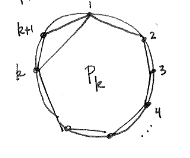
\includegraphics[width=100]{Midterm two/screenshot_2017-03-03_16-17-22.png}
\end{center} Imagine, any number of
edges \(k\), where the first edge is named 1. One could simply add another
\(k+1\) edge to the list.

\item \uline{Example}: Prove that any \(2^n\times2^n\) grid of squares with any one
square removed can be tiled with \emph{L}-shaped tiles.

\begin{figure}[htbp]
\centering
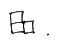
\includegraphics[width=50]{Midterm two/screenshot_2017-03-03_15-48-14.png}
\Leftarrow\textit{L-shaped tiles}
\end{figure} Removing any box
results in the remaining boxes being an \emph{L}-shaped tile.

\begin{figure}[htbp]
\centering
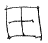
\includegraphics[width=50]{Midterm two/screenshot_2017-03-03_16-00-29.png}
\Leftarrow\textit{box}
\end{figure} 

\begin{center}
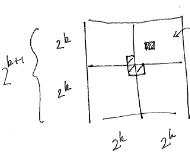
\includegraphics[width=125]{Midterm two/screenshot_2017-03-03_16-01-43.png}
\end{center} A large block can be
covered by \emph{L}-shapes by hypothesis. What about other 3 blocks?

Inductive hypothesis doesn't apply to grid \(2^k\times2^k\) \uline{without}
removing a square. Meaning without removing one atomic box.

\uline{Solution}: consider removing a single \emph{L} instead, taking away a box from
three quadrants. It is an equivalent procedure.
\end{itemize}

\subsection{Ordered Fields}
\label{sec:orgd1c9494}
\begin{definition}{Axioms of an Ordered Field}
  We begin by assuming the existence of a set \Real, called the set of real
  numbers, and two operations ``+'' and ``$\cdot$'', called addition and
  multiplication, such that the following properties apply :---
  \begin{itemize}
  \item [A1. ] For all $x,y \in \Real$, $x + y \in \Real$ and if $x = w$ and $y
    = z$, then $x + y = w + z$.
  \item [A2. ] For all $x,y \in \Real$, $x + y = y + x$.
  \item [A3. ] For all $x,y,z \in \Real$, $x + (y + z) = (x + y) + z$.
  \item [A4. ] There is a unique real number $0$ such that $x + 0 = x$, for all
    $x \in \Real$.
  \item [A5. ] For each $x \in \Real$ there is a unique real number $-x$ such
    that $x + (-x) = 0$.
  \item [M1. ] For all $x,y \in \Real$, $x \cdot y \in \Real$ and if $x = w$ and
    $y = z$, then $x \cdot y = w \cdot z$.
  \item [M2. ] For all $x,y \in \Real$, $x \cdot y = y \cdot x$.
  \item [M3. ] For all $x,y,z \in \Real$, $x \cdot (y \cdot z) =(x \cdot y)
    \cdot z$.
  \item [M4. ] There is a unique real number $1$ such that $1 \ne 0$ and $x
    \cdot 1 = x$ for all $x \in \Real$.
  \item [M5. ] For each $x,y \in \Real$ with $x \ne 0$, there is a unique real
    number $1/x$ such that $x \cdot (1/x) = 1$. We also write $x^{-1}$ or
    $\frac{1}{x}$ in place of $1/x$.
  \item [DL. ] For all $x,y,z \in \Real$, $x \cdot (y + z) = x \cdot y + x \cdot
    z$.
  \end{itemize}
  \begin{remark}
    These first 11 axioms are called the field axioms because they describe a
    system know as a field in the study of abstract algebra. Axioms A2 and M2
    are called the \textit{\textbf{commutative laws}} and axioms A3 and M3 are
    the \textit{\textbf{associative laws}}. Axiom DL is the
    \textit{\textbf{distributive law}} that shows how addition and
    multiplication relate to each other. Because of A1 and M1, we can think of
    addition and multiplication as functions that map $\Real \times \Real$ into
    $\Real$. When writing multiplication we often omit the raised dot and write
    $xy$ instead of $x \cdot y$.
  \end{remark}
  In addition to the field axioms, the real numbers also satisfy four order
  axioms.
  \begin{itemize}
  \item [O1. ] For all $x,y \in \Real$, exactly one of the relations $x = y$, $x
    > y$, or $x < y$ holds (\textit{\textbf{trichotomy law}}).
  \item [O2. ] For all $x,y,z \in \Real$, if $x < y$ and $y < z$, then $x < z$.
  \item [O3. ] For all $x,y,z \in \Real$, if $x < y$, then $x + z < y + z$.
  \item [O4. ] For all $x,y,z \in \Real$, if $x < y$ and $z > 0$, then $xz <
    yz$.
  \end{itemize}
\end{definition}

\begin{definition}{Absolute Value}
  \label{Absolute Value}
  If $x \in \Real$, then the absolute value of $x$, denoted by $\abs{x}$, is
  defined by :---
  $$\abs{x} =
  \begin{cases}
    x, & $if $ x\ge 0, \\
    -x, & $if $ x\le 0.
  \end{cases}$$

  Let $x,y \in \Real$ and let $a \ge 0$. Then
  \begin{itemize}
  \item [(a) ] $\abs{x} \ge 0$,
  \item [(b) ] $\abs{x} \le a$ iff $-a \le x \le a$,
  \item [(c) ] $\abs{xy} = \abs{x} \cdot \abs{y}$,
  \item [(d) ] $\abs{x + y} \le \abs{x} + \abs{y} $.
  \end{itemize}
  \begin{remark}
    Part (d) of \textbf{Def \ref{Absolute Value}} is referred to as the
    \textit{\textbf{triangle inequality}}, and has other forms. For example,
    letting $x = a - c$ and $y = c - b$, we obtain $$\abs{a - b} \le \abs{ a -
      c} + \abs{c - b}$$
  \end{remark}
\end{definition}

\subsection{Completeness Axiom}
\label{sec:org02f2ffe}
\begin{definition}{Irrational.}
  Let $p$ be a prime number. Then $\sqrt{p}$ is not a rational number.
\end{definition}

\begin{definition}{Bounds.}
  Let $S$ be a subset of $\Real$. If there exists a real number $m$ such that
  $m\ge s$ for all $s\in S$, then $m$ is called an \textit{\textbf{upper bound}}
  of $S$, and we say that $S$ is bounded above. If $m\le s$ for all $s\in S$,
  then $m$ is a \textit{\textbf{lower bound}} of $S$ and $S$ is bounded below.
  The set $S$ is said to be \textit{\textbf{bounded}} if it is bounded above and
  bounded below.
\end{definition}

\begin{definition}{Maximum and Minimum.}
  If an upper bound $m$ of $S$ is a member of $S$, then $m$ is called the
  maximum (or largest element) of $S$, and we write $$m=\text{max } S.$$
  Similarly, if a lower bound of $S$ is a member of $S$, then it is called
  the \textit{\textbf{minimum}} (or least element) of $S$, denoted by
  $$m=\text{min } S.$$
\end{definition}

\begin{definition}{Supremum and Infimum.}
  Let $S$ be a nonempty subset of $\Real$. If $S$ is bounded above, then the least
  upper bound of $S$ is called its \textit{\textbf{supremum}} and is denoted
  by $\text{sup } S$. Thus $m=\text{sup } S$ iff
  \begin{enumerate}
    \item $m \ge s$, for all $s \in S$, and 
    \item if $m\pr < m$, then there exists $s\pr \in S$ such that $s\pr > m\pr$.
  \end{enumerate}
  If $S$ is bounded below, then the greatest lower bound of $S$ is called its
  \textit{\textbf{infimum}} and is denoted by $\text{inf } S$, so
  $m=\text{inf } S$.
\end{definition}

\begin{definition}{Completeness Axiom.}
  Every nonempty subset $S$ of $\Real$ that is bounded above has a least upper
  bound. That is, $\text{sup } S$ exists and is a real number.
\end{definition}

\begin{definition}{Archimedean Property of $\Real$.}
  The set $\Natural$ of natural numbers is unbounded above in $\Real$.
\end{definition}

\begin{definition}{Density of $\Rational$ in $\Real$}
  If $x$ and $y$ are real numbers with $x < y$, then there exists a rational
  number $r$ such that $x < r < y$.
\end{definition}

\subsection{Boundaries}
\label{sec:org451612e}
\begin{definition}{Neighborhood.}
  Let $x\in\Real$ and let $\varepsilon>0$. A \textit{\textbf{neightborhood}}
  of $x$ (or an \textit{\textbf{$\varepsilon$-neightborhood}} of $x$) is a
  set of the form $N(x; \varepsilon)=\{y\in\Real : \abs{x-y}<\varepsilon\}$.
  \begin{remark}
    The professor uses the notation: $$N_\varepsilon(x)=\{y\in\Real :
    \abs{x-y}<\varepsilon\},$$ which is probably nicer.
  \end{remark}
\end{definition}

\begin{definition}{Deleted Neighborhood.}
  Let $x\in\Real$ and let $\varepsilon>0$. A \textit{\textbf{deleted
      neighborhood}} of $x$ is a set of the form $N^*(x;\varepsilon)=\{y\in\Real
  : 0<\abs{x-y}<\varepsilon\}$. Clearly, $N^*(x;\varepsilon) =
  N(x;\varepsilon)\setminus\{x\}$
  \begin{remark}
    The professor uses the notation: $$N_\varepsilon^*(x)=\{y\in\Real :
    0<\abs{x-y}<\varepsilon\},$$ which is probably nicer.
  \end{remark}
\end{definition}

\begin{definition}{Open and Closed Sets.}
  Let $S \sube \Real$. If $\bd{S} \sube S$, then $S$ is said to be
  \textit{\textbf{closed}}. If $\bd{S} \sube \Real \setminus S$, then $S$ is
  said to be \textit{\textbf{open}}.
\end{definition}

\subsection{Theorem}
\label{sec:org80cd39a}
\begin{itemize}
\item The union of open sets is open.
\item The intersection of finitely-many open sets is open.
\end{itemize}
\subsubsection{Section 3.3}
\label{sec:orgccdc12a}
\section{Midterm three}
\label{sec:orga479a4c}
\subsection{Topology of the Real Numbers}
\label{sec:org719fdb4}
Every bounded sequence has a convergent subsequence.
\begin{itemize}
\item If \(\{s_n\}\) bounded, then
\begin{enumerate}
\item for every \(\varepsilon\), \(\exists N \in \Natural \ni s_n < m + \varepsilon\) when \(n \ge N\).
(Else there are infinitely many \(s_n \ge m + \varepsilon\), so there can't
be a lim sup.)
\item for every \(\varepsilon > 0\), \(\forall i \in \Natural, \exists k>i\) with \(s_k > m - \varepsilon\).
(There are infinitely many \(s_k \in (m-\varepsilon, m+\varepsilon)\), else
\(m-\varepsilon\) is upper bound for all limits of subsequences.)
\end{enumerate}
\end{itemize}

\begin{definition}{Open and Closed Sets.}
  Let $S \sube \Real$. If $\bd{S} \sube S$, then $S$ is said to be
  \textit{\textbf{closed}}. If $\bd{S} \sube \Real \setminus S$, then $S$ is
  said to be \textit{\textbf{open}}.

  $S$ is closed $\iff$ $S$ contains all of its accumulation points $\iff$ its
  complement $\Real \setminus S$ is open $\iff S =$ cl $S$.

  A set $S$ is open $\iff$ $S =$ int $S$ $\iff$ every point in $S$ is an
  interior point of $S$.
\end{definition}

\begin{definition}{Interior Point and Boundary Point.}
  Let $S$ be a subset of $\Real$. A point $x$ in $\Real$ is an
  \textit{\textbf{interior point}} of $S$ if there exists a neighborhood $N$
  of $x$ such that $N \sube S$. If for every neighborhood $N$ of $x$, $N \cap
  S \ne \varnothing$ and $N \cap (\Real \setminus S) \ne \varnothing$, then $x$ is called a
  \textit{\textbf{boundary point}} of $S$. The set of all interior points of
  $S$ is denoted by int $S$, and the set of all boundary points of $S$ is
  denoted by $\bd{S}$.
\end{definition}

\begin{definition}{Accumulation Points.}
  Let $S$ be a subset of $\Real$. A point $x$ in $\Real$ is an
  \textbf{accumulation point} of $S$ if every deleted neighborhood of $x$
  contains a point of $S$. That is, for every $\varepsilon > 0$, $N^{*}(x,\varepsilon) \cup S \ne
  \varnothing$. The set of all accumulation points of $S$ is denoted by
  $S\pr$. If $x\in S$ and $x\notin S\pr$, then $x$ is called an \textbf{isolated
  point} of $S$.
\end{definition}

\begin{definition}{Closure.}
  Let $S \sube \Real$. Then the closure of $S$, denoted $\text{cl } S$, is
  defined by $$\text{cl } S = S \cup S\pr,$$ where $S\pr$ is the set of all
  accumulation points of $S$.

  Also, $$\text{cl } S = S \cup \text{bd } S.$$
\end{definition}

\subsection{Compact Sets}
\label{sec:org022bae4}
\begin{definition}{Compact, Open Cover, and Subcover.}
  A set $S$ is said to be \textit{\textbf{compact}} if whenever it is
  contained in the union of a family $\F$ of open sets, it is contained in
  the union of some finite number of the sets in $\F$. If $\F$ is a family of
  open sets whose union contains $S$, then $\F$ is called an
  \textit{\textbf{open cover}} of $S$. If $\G \sube \F$ and $\G$ is also an open
  cover of $S$, then $\G$ is called a \textit{\textbf{subcover}} of $S$.

  \begin{corollary}{}
      $S$ is compact $\overset{Heine-Borel}{\iff}$ $S$ is closed and bounded
      $\iff$ every infinite subset of S has an accumulation point in $S$.

      $S$ is a nonempty closed bounded subset of $\Real$ $\Rightarrow$ $S$ has a maximum
      and a minimum.
  \end{corollary}
\end{definition}

\begin{definition}{Heine--Borel.}
  A subset $S$ of $\Real$ is compact iff $S$ is closed and bounded.
\end{definition}

\begin{definition}{Bolzano--Weierstrass.}
  If a bounded subset $S$ of $\Real$ contains infinitely many points, then there
  exists at least one point in $\Real$ that is an accumulation point of $S$.
\end{definition}

\subsection{Sequences}
\label{sec:org2fa21a3}
\begin{definition}{Sequence.}
  A sequence $S$ is a function whose domain is the set $\Natural$ of natural
  numbers. Denoted by its value of $n$ at $s_n$ instead of $S(n)$ or by listing
  its values $(s_1, s_2, s_3, ...)$. $s_n$ is the $n^{th}$ term of the sequence.
\end{definition}

\begin{definition}{Convergence, Divergence, Limit.}
  A sequence $(s_n)$ is said to \textbf{\textit{converge}} to the real number
  $s$ provided that
  \begin{center}
    for every $\varepsilon > 0$ there exists a natural number $N$ such that for
    all $n \in \Natural$, $n \ge N$ implies that $\abs{s_n - s} < \varepsilon$.
  \end{center}
  If $(s_n)$ converges to $s$, then $s$ is called the \textbf{\textit{limit}}
  of the sequence $(s_n)$, and we write $\underset{n\rightarrow\infty}{\text{lim}} s_n = s$,
  lim $s_n = s$, or $s_n \rightarrow s$. If a sequence does not converge to a real
  number, it is said to \textbf{\textit{diverge}}.
\end{definition}

\begin{definition}{Subsequence.}
Let $(s_n)_{n=1}^\infty$ be a sequence and let $(n_k)_{k=1}^{\infty}$ be any sequence
of natural numbers such that $n_1 < n_2 < ...$. The sequence
$(s_{n_k})_{k=1}^{\infty}$ is called a \textit{\textbf{subsequence}} of
$(s_n)_{n=1}^\infty$.
\end{definition}

\begin{definition}{Limit Superior and Limit Inferior.}
  Let $(s_n)$ be a bounded sequence. A \textbf{\textit{subsequential limit}}
  of $(s_n)$ is any real number that is the limit of some subsequence of
  $(s_n)$. If $S$ is the set of all subsequential limits of $(s_n)$, then we
  define the \textbf{\textit{limit superior}} (or \textbf{\textit{upper
  limit}}) of $(s_n)$ to be $$\text{lim sup } s_n = \text{sup } S.$$
  Similarly, we define the \textit{\textbf{limit inferior}} (or
  \textit{\textbf{lower limit}}) of $(s_n)$ to be $$\text{lim inf } s_n =
  \text{inf } S.$$
\end{definition}

\begin{definition}{Bounded Sequence.}
  A sequence $(s_n)$ is said to be \textit{\textbf{bounded}} if the range $\{
  s_n : n \in \Natural \}$ is a bounded set, that is, if there exists an $M \ge
  0$ such that $\abs{s_n} \le M$ for all $n \in \Natural$

  Every convergent sequence is bounded.

  If a sequence converges, its limit is unique.

  Every bounded sequence has a convergent subsequence.
\end{definition}

\subsection{Limit Theorem}
\label{sec:org456a7bd}
\begin{definition}{Limit Theorems.}
  \begin{enumerate}
    \item $\lim{(s_n + t_n)} = s + t$
    \item $\lim{(ks_n)} = ks$ and $\lim{(k + s_n)} = k + s$, for any $k \in
      \Real$
    \item $\lim{(s_n t_n)} = st$
    \item $\lim{(s_n/t_n)} = s/t$, provided that $t_n \ne 0$ for all $n$ and $t
      \ne 0$
  \end{enumerate}
\end{definition}

\begin{definition}{Lesser Convergence.}
  Suppose that $(s_n)$ and $(t_n)$ are convergent sequences with $\lim{s_n} =
  s$, and $\lim{t_n} = t$. If $s_n \le t_n$ for all $n \in \Natural$, then $s
  \le t$.
\end{definition}

\begin{corollary}
  If $(t_n)$ converges to $t$ and $t_n \ge 0$ for all $n \in \Natural$, then $t
  \ge 0$.
\end{corollary}

\begin{definition}{Ratio Convergence.}
  Suppose that $(s_n)$ is a sequence of positive terms and that the sequence of
  rations $(s_{n+1} / s_n)$ converges to $L$. If $L < 1$, then $\lim{s_n} = 0$
\end{definition}

\begin{definition}{Divergence.}
  A sequence $(s_n)$ is said to \textit{\textbf{diverge to}} $+\infty$, and we
  write $\lim{s_n} = +\infty$ provided that
  \begin{center}
    for every $M \in \Real$ there exists a natural number $N$ such that $n \ge
    N$ implies that $s_n > M$.
  \end{center}

  A sequence $(s_n)$ is said to \textit{\textbf{diverge to}} $-\infty$, and we
  write $\lim{s_n} = +\infty$ provided that
  \begin{center}
    for every $M \in \Real$ there exists a natural number $N$ such that $n \ge
    N$ implies that $s_n < M$.
  \end{center}
\end{definition}

\begin{definition}{Greater Divergence.}
  Suppose that $(s_n)$ and $(t_n)$ are sequences such that $s_n \le t_n$ for all
  $n \in \Natural$.
  \begin{enumerate}
    \item If $\lim{s_n} = +\infty$, then $\lim{t_n} = +\infty$.
    \item If $\lim{t_n} = -\infty$, then $\lim{s_n} = -\infty$.
  \end{enumerate}
\end{definition}

\begin{definition}{Inverse of Divergence.}
Let $(s_n)$ be a sequence of positive numbers. Then $\lim{s_n} = +\infty$ $\iff$
$\lim{(1/s_n)} = 0$.
\end{definition}

\subsection{Monotone Sequences and Cauchy Sequences}
\label{sec:orgecca96d}
\begin{definition}{Monotone Sequences.}
  A sequence $(s_n)$ of real numbers is \textit{\textbf{increasing}} if $s_n \le
  s_{s_n+1}$ for all $n \in \Natural$ and is \textit{\textbf{decreasing}} if
  $s_n \ge s_{n+1}$ for all $n \in \Natural$. A sequence is
  \textbf{\textit{monotone}} if it is increasing or decreasing.
\end{definition}

\begin{definition}{Monotone Convergence Theorem}
  A monotone sequence is convergent $\iff$ it is bounded.
\end{definition}

\begin{definition}{Cauchy Sequence}
If, for every $\varepsilon>0$, there exists $N \in \Natural$ such that if $m,n \ge N$ then
$\abs{s_n - s_m} < \varepsilon$.

Every convergent sequence is \textit{\textbf{Cauchy}}.

If $(s_n)$ is a \textit{\textbf{Cauchy}} sequence, then $(s_n)$ converges.
\end{definition}

\begin{proof}
   Given any $\varepsilon > 0$, choose $N$ such that $\abs{s_n - s} < \frac{\epsilon}{2}$ if
  $n \ge N$ (which is possible to do since $s_n \rightarrow s$). Then $\abs{s_n - s_m} =
  \abs{s_n - s + s - s_m}$ because adding and subtracting by the limit is the
  same as doing nothing, and, by the triangle inequality, $\abs{s_n - s + s -
  s_m} \le \abs{s_n - s} + \abs{s_m - s} < \frac{\varepsilon} + \frac{\varepsilon}$.
\end{proof}
\end{document}